\documentclass[a4paper, oneside]{report}

\usepackage[vlined, ruled, linesnumbered]{algorithm2e}
\usepackage{amsmath}
\usepackage{fancyref} % Better reference.

\usepackage{pdflscape} % Gør landscape-environmentet tilgængeligt
\usepackage{fixme} % Indsæt "fixme" noter i drafts.
%\usepackage{hyperref} % Indsæter links (interne og eksterne) i PDF

\usepackage[format=hang]{caption,subfig}
\usepackage{graphicx}
%\usepackage{stmaryrd}
\usepackage{amssymb}
%\usepackage{listings}
%\usepackage{ulem} % \sout - strike-through
%\usepackage{tikz}
\renewcommand{\ttdefault}{txtt} % Bedre typewriter font
\newcommand{\keyword}{\ttfamily}
\newcommand{\STL}{STL (C++ Standard Template Library)~}

\setcounter{secnumdepth}{-1} % Sæt overskriftsnummereringsdybde. Disable = -1.
\newcommand{\projecttitle}{Implementing and parallelising Bursttries}

\title{\projecttitle}
\author{Jacob Wejendorp}
%\renewcommand{\bibsection}{\section*{References}}
\begin{document}
\maketitle
\begin{abstract}
With the scaling of CPUs focusing more on increases in the number of cores,
highly parallelisable data structures are of increasing importance.

This project seeks to explore the implementation tradeoffs in parallelising the
burst trie data structure, which has been shown to be on par with hash maps in
both speed and space consumption. The burst trie provides fast access to
strings and integers, however different bucket types have different advantages
and disadvantages.

By comparing different tradeoffs needed to implement partial functionalities,
specialized data structures are developed. Depending on the level of
parallelism, distribution of insertions/searches/removals, and the
distribution of the inserted data, different variations excel. This means
evaluating the modifications needed to make the trie work as a threadsafe set-,
multiset- or map container.

The performance of the trie in sequential testing is found to degrade with
increased bucket sizes, while the opposite tendency is found for parallel
scaling for larger datasets. As such no silver bullet is found for bucket
sizes.

Using a relatively simple locking mechanism, speedups of up to a factor $6$ are
observed for searches and $3.5$ for insertions, when utilizing 8 CPUs.

A lock-free implementation technique is proposed to avoid bottlenecking at the
root, but not successfully implemented.

\end{abstract}

\clearpage

\tableofcontents
%\listoftables
%\listoffigures
\clearpage

\chapter{Introduction}

\section{Problem definition}
How can the burst trie be parallelised in a way that allows building and searching
the structure faster than an equivalent serial singlethreaded approach?
What kind of overhead does it create, and does this influence relative
performance between the individual variants of the structure?


\section{Background}
%Define: What is a trie?
A trie is a data structure for storing keys based on their prefixes.
It is also known as a prefix-tree. The idea is equivalent to that of
"most significant digit" (MSD-)radix sort.

At each level in the tree a prefix of the key is read and branches performed
accordingly. A trie working on strings with the ASCII alphabet will thus have a
branching factor of 128. The character that is read corresponds to a branch in
the current node. This branching moves down another level in the trie until
finding the leaf matching the requested key or terminating unsuccesfully. A
trie is as deep as the longest key that it contains, since each level removes a
character from the key. It is this bound that newer trie variants attempt to
improve, without compromising lookup efficiency.

%Define: What is the idea of a burst trie?
Following the radix sort analogy, the regular trie uses radix-sort until
reaching the trivial case, with no boundary for using other sorting methods.
The burst trie on the other hand, uses a limit for employing other methods
based on the element count. In other words a burst trie differs from a regular
trie by compressing the elements into so-called bucket structures when
there are few of them in a particular subtree. Each bucket is then assigned a
capacity. When inserting elements into a burst trie, the structure finds the
corresponding bucket and puts the element in it. If the bucket exceeds its
capacity it "bursts", creating a new parenting node and redistributing the
elements into buckets under it, based on the next part of the prefix. As such,
each bucket is uniquely determined by its prefix (or path in the trie). The
elements in each bucket therefore all have the same prefix, making it possible
to discard this part of the key to save space. This is what makes it possible
for the trie to be more space efficient than an equivalent hashmap, or
    comparison-based tree structure.

% Why are burst tries nice?
Burst tries have been shown to be faster and more space efficient than
compari\-son-based data structures such as B-trees and red-black trees when used
on integer data\cite{Nash:2008}. For strings the burst trie is more efficient
than trees\cite{Heinz:2002} while unlike hash-tables allowing efficient iteration
of sorted keys with minor modifications. These modifications are one of the
focus areas of this project.

The original burst trie uses linked lists for the containers, but this has been
shown to be inefficient in a modern cache hierachy. There has been done research
in different ways to improve the structure, by replacing the bucket structure.
Nash \& Gregg have done work on optimizing the trie itself, using so-called
level- and path-compression\cite{Nash:2008}. More complex tries exist in
the forms of both Judy and Patricia tries. They work by dynamically changing
the bucket types depending on load, and using different metrics to compress
the trie itself, but are more sensitive to skew data distributions.

In an earlier course, the author has done work on the burst trie as an Integer
data structure\cite{Wejendorp:2010} in cooperation with Niels Grathwohl. There,
a simplistic bit-string approach was used to treat integers as bit-strings when
branching in an attempt to implement parts of, and verify the results of Nash
\& Gregg\cite{Nash:2008}. That work is extended in this project in the form of
investigating a wider range of solutions for each addition to the basic trie.

% Multithreading!! - The open problem!
While maintaining optimizations for caching remains important, modern processor
scaling primarily focuses on multithreading, making it increasingly important
to create efficient multi-threaded data structures and algorithms. To the
author's knowledge, no work has been done on parallelising the structure for
modern multi-core processors, as this was left open by Askitis and Sinha in
\cite{Askitis:2010}. The goal of this project is therefore specifically
parallelising the structure in a way that allows insertions and deletions
faster than the sequential implementation, while remaining space
efficient\cite{Askitis:2010}. This means evaluating the sacrifices needed to
make the structure threadsafe; the number of locks, indicator variables and the
like.

Parallelism in general is a very complex issue, with cache alignment having a
potentially large impact on performance, from so-called false sharing
\cite{Shavit:2011}. This phenomenon occurs when two CPUs operate on the same
memory region, but on independent data, and is the unnecessary synchronization
of cache lines between CPUs.

Another area of interest is minimal locking, which will decrease the amount of
syncrhonization between threads. The standard data structures of C++ are all
threadsafe in terms of concurrent reads, but not writes. As such, a simple
read/write lock can be used to wrap the structure, causing forced sequential
writing, while allowing multiple readers. When locks are used, the scheduler
must guarantee that the threads holding the locks are not preempted. Otherwise
the performance of all waiting threads will suffer. A solution to this is to
try and design a lock-free implementation.\cite{Shavit:2011}

What makes lock-free implementation difficult is potential race conditions from
data dependencies. This is attempted to be resolved using a
mixture of so-called atomic operations, in combination with compare-and-swap
(CAS) and contention. Using this method, one operation will always succeed for
every time another fails, and progress is guaranteed regardless of what the
scheduler does\cite{Shavit:2011}.

It is therefore of great interest to investigate ways to make the trie lock-free.
Doing so will also ensure operations not being limited in terms of parallelisation
by the granularity of the locking mechanisms.

\chapter{Implementation}
By first establishing the regular trie methods, a basis is made for evaluating
the modifications required by the other types.

\section{Generic Trie}

\begin{algorithm}[H]
    \caption{\FuncSty{Insert(}$k$\FuncSty{)}}
    $Node \leftarrow$  root node\;
    \ForEach{char $c$ in $k$}{
        \eIf{$Node$ has child $c$}{
            $Node \leftarrow Node[c]$\;
        }{ %else
            \emph{Create $Node[c]$}\;
            $Node \leftarrow Node[c]$\;
        }
    }
    \emph{Set end of string flag on $Node$}\;
\end{algorithm}
Using this as the basis for the insertion and deletion methods, the trie is
built and searched by reading one character at a time. So just like an
insertion might create a deep path down the trie, a deletion will have to
remove dead ends, upon removing an entry.

A depth-first approach is taken with deletions. The recursive call returns with
a value, determining if changes might be needed at the higher level.


With the nodes having $\alpha$ pointers, the memory overhead for sparse tries
is very big.

As a function of collision odds, each unique subtrie incurs $(\alpha-1) l$
pointers of overhead for a unique substring of length $l$. As such, the total
pointer count is anywhere up to:
\begin{align*}
    M(n) = O(n * (\alpha l - 1))\\
\end{align*}
Which will be used as baseline for comparisons.

The cost of insertion is a function of the chance that a string is unique on
each level. The first insertion has 0 chance of being non-unique, creating a
base-case costing $\alpha$ new pointers in the created subnode.
\[
    T(n) = \left\{ \begin{array}{ll}
                    (\frac{\alpha - 1}{\alpha})^m           & \text{if } n = 1 \\
                    T(n-1) + (\frac{\alpha - 1}{\alpha})^m   & \text{if } n > 1
                   \end{array}
                \right.
\]
For the m'th insertion of an n-length word to the node.




\section{Burst trie}
Based on the descriptions in \cite{Nash2008}, the algorithms for search
and insertion are as such:

\begin{algorithm}[H]
    \caption{\FuncSty{Search(}$k$\FuncSty{)}}
    \label{alg:bt_search}

    $Node \leftarrow$  root node\;
    \ForEach{char $c$ in $k$}{
        \eIf{$Node$ has child $c$}{
            $Node \leftarrow Node[c]$\;
        }{ %else
            \eIf{$Node$ has bucket $B[c]$}{
                \emph{Lookup remaining $k$ in $B[c]$}\;
            }{
                \Return{Nothing}\;
            }
        }
    }
\end{algorithm}

where the lookup phase depends on the bucket structure chosen. The original
lookup uses sorted doubly-linked lists. 

\begin{algorithm}[H]
    \caption{\FuncSty{Insert(}$k$\FuncSty{)}}
    \label{alg:bt_insert}

    \SetKwFunction{Burst}{burst}

    $Node \leftarrow$  root node\;
    \tcp{Move down until reaching bucket reference}
    \ForEach{char $c$ in $k$}{
        \If{$Node$ has child $c$}{
            $Node \leftarrow Node[c]$\;
        }
    }
    \tcp{Node either has a bucket at $c$ or one is created}
    \eIf{$Node$ has bucket $B[c]$}{
        \emph{Insert remaining $k$ in $B$}\;
        \If{$B$ is full}{
            $Node[c] \leftarrow \Burst(B)$\;
        }
    }{
        $b \leftarrow $\emph{Create bucket and insert $k$}\;
    }
\end{algorithm}

Deletions are mentioned to be equivalent to insertions, in that removing a key
may cause removal of a bucket, and nodes. The method being equivalent to that
of the basic trie, or the insertion algorithm in reverse.

\begin{algorithm}[H]
    \caption{\FuncSty{Burst(}$b$\FuncSty{)}}
    \label{alg:bt_burst}

    \ForEach{value $k,v$ in $b$}{
        \If{$Node$ has child $c$}{
            $Node \leftarrow Node[c]$\;
        }
    }
\end{algorithm}


\subsection{Bucket structures}
% Advantages
% Disadvantages
% Time bounds
Depending on the chosen bucket structure, insertions, deletions and searches
accomplish different time complexities, and allow different bucket sizes
without becoming inefficient.
An added dimension to this research when compared to previous attempts is the
changes needed to make each container threadsafe.

\subsubsection{Linkedlists}
% Advantages
Easy to maintain. Constant time insertions.
If the linkedlist is maintained with a {\keyword head} and {\keyword tail} pointer,
and kept single-linked, insertions using a simple {\keyword AO\_compare\_and\_swap}
pointer-swap.

% Disadvantages
A linked-list is known for its bad cache locality, which makes it slow in
searches and iterations when compared to an array implementation, despite
having the same time bounds. A linkedlist is a pointer-based bucket, making
random-acccess impossible, resulting in limited options for searching and
sorting. Assuming a worst-case allocation scenario, a traversal of the bucket
incurs up to $b$ cache misses in a per-node allocation scheme.

% Space consumption
The space consumption of linkedlists are equivalent to that of a binary tree,
if a doubly-linked list is used, or one pointer less per entry for a
single-linked list.

% Time bounds
\begin{table}[h!]
    \centering
    \begin{tabular}[here]{ r || c | c | c}
        Operation & Average case & Worst case & Requires locking  \\ \hline
        Insert    & $O(1)$ & $O(1)$   & C  \\ \hline
        Delete    & $O(n)$ & $O(n)$   & E \\ \hline
        Find      & $O(n)$ & $O(n)$   & C  \\ \hline
    \end{tabular}
    \caption{Time bounds for the bucket operations using unsorted linkedlists,
    $n$ denoting number of elements in the list. Locking terms use E for
        exclusive and C for concurrent.}
    \label{tab:bounds:linkedlist}
\end{table}
The find and insert operations can be kept separate from delete by using a
read-lock.

\subsubsection{Binary search tree}
% Advantages
The binary search trees allow for a (average case) logarithmic insertion,
search and deletion structure. This was found to be the optimal
bounds\cite{Nash2008}.

So the binary search trees are theoretically optimal, while having little space
overhead.

% Disadvantages
However, the binary search trees were found to be inefficient due to caching,
being a pointer-based bucket structure. A basic binary search tree has no
guarantees on the height, which is based on the insertion order. This doing a
pre-order tree-walk when bursting, preserving the insertion order, on the next
part of the key.

%Space consumption
The binary search trees will only use 2 pointers per element, and
has no overhead from preallocation. 

% Time bounds
\begin{table}[h!]
    \centering
    \begin{tabular}[here]{ l || c | c | c}
        Operation & Average case & Worst case & Requires locking  \\ \hline
        Insert    & $O(\log n)$ & $O(n)$ & E \\ \hline
        Delete    & $O(\log n)$ & $O(n)$ & E \\ \hline
        Find      & $O(\log n)$ & $O(n)$ & C  \\ \hline
    \end{tabular}
    \caption{Time bounds for the bucket operations using binary search trees,
    $n$ denoting number of elements in the bucket. Locking terms use E for
        exclusive and C for concurrent.}
    \label{tab:bounds:linkedlist}
\end{table}
The find and insert operations can be kept separate from delete by using a
read-lock.

\subsubsection{Arrays}
% Advantages
Advantages of using arrays are primarily cache-efficiency, since the
elements can be stored in one consecutive memory segment.
However.. shared cache-lines (ACM article) ... might be a problem with parallelism?

% Disadvantages
When using arrays, however, a tradeoff between efficient insertions or
efficient searches will have to be made. A sorted array is the most compressed
logarithmic time searchable representation of the elements. This makes for
cache- and time-efficient searching of the buckets, while increasing the
insertion cost to become worst case linear in the bucket size, with bigger
constant factors from reallocations.

% Space consumption
If dynamic arrays are used, a 2-approximation can be maintained, meaning the
overhead will be within a factor 2 of the elements' total size, having no
extra pointers to maintain.

Another approach is to allocate the full bucket capacity, possibly creating a
factor B waste.

% Time bounds
This means that either insertion or searching will be linear in the bucket
size, and therefore define the limit on the desired bucket size.

\begin{table}[h!]
    \centering
    \begin{tabular}[here]{ l || c | c | c}
        Operation & Average case & Worst case & Requires locking  \\ \hline
        Insert    & $O(1)$ & $O(1)$ & E \\ \hline
        Delete    & $O(n)$ & $O(n)$ & E \\ \hline
        Find      & $O(n)$ & $O(n)$ & C  \\ \hline
    \end{tabular}
    \caption{Time bounds for the bucket operations using unsorted static
    arrays, $n$ denoting number of elements in the bucket. Insertion might be
    linear because of dynamic resizing of the array. Locking terms use E for
        exclusive and C for concurrent.}
    \label{tab:bounds:unsortedarray}
\end{table}
\begin{table}[h!]
    \centering
    \begin{tabular}[here]{ l || c | c | c}
        Operation & Average case & Worst case & Requires locking  \\ \hline
        Insert    & $O(1)$ & $O(n)$ & E \\ \hline
        Delete    & $O(n)$ & $O(n)$ & E \\ \hline
        Find      & $O(n)$ & $O(n)$ & C  \\ \hline
    \end{tabular}
    \caption{Time bounds for the bucket operations using unsorted dynamic
    arrays, $n$ denoting number of elements in the bucket. Insertion might be
    linear because of dynamic resizing of the array. Locking terms use E for
        exclusive and C for concurrent.}
    \label{tab:bounds:unsortedarray}
\end{table}
\begin{table}[h!]
    \centering
    \begin{tabular}[here]{ l || c | c | c}
        Operation & Average case & Worst case & Requires locking  \\ \hline
        Insert    & $O(n)$ & $O(n)$           & E \\ \hline
        Delete    & $O(n)$ & $O(n)$           & E \\ \hline
        Find      & $O(\log n)$ & $O(\log n)$ & C  \\ \hline
    \end{tabular}
    \caption{Time bounds for the bucket operations using binary search trees,
    $n$ denoting number of elements in the bucket. Locking terms use E for
        exclusive and C for concurrent.}
    \label{tab:bounds:sortedarray}
\end{table}


\subsubsection{Hash tables}
%Advantages
The idea of using hash tables as an intermediate step is dubbed a HAT-trie,
and using bit-wise hashing creates sub-buckets, allowing the buckets
as a whole to become very large without becoming inefficient to access.

%Disadvantages
This presents the issue of creating an efficient hashing function with
low collision rate. That is, finding the ballance between having $B$
hash containers, which is essentially just another level of nodes, and
the number of collisions resulting in skewed distributions of values amongst
the sub-buckets. 

This concept is further covered in Zobel et al. 2005, which covers cache conscious
hash tables. This means that the buckets can be very large, reducing the number of
nodes created in the trie over all, and with a cache-efficient bucket structure
the overall outcome should be very fast.


% Space consumption
Hash tables have a relatively large overhead of lookup tables and stuff...
\fxnote{TODO Look into hash tables!}

%Time bounds
\begin{table}[h!]
    \centering
    \begin{tabular}[here]{ l || c | c | c}
        Operation & Average case & Worst case & Requires locking  \\ \hline
        Insert    & $O(\log n)$ & $O(\log n)$ & E \\ \hline
        Delete    & $O(\log n)$ & $O(\log n)$ & E \\ \hline
        Find      & $O(\log n)$ & $O(\log n)$ & C \\ \hline
    \end{tabular}
    \caption{Time bounds for the bucket operations using hashmaps,
    $n$ denoting number of elements in the bucket. Locking terms use E for
        exclusive and C for concurrent.}

    \label{tab:bounds:hashmap}
\end{table}

\clearpage
\section{STL conformity}
Using the STL containers for reference, the implementation will have to include
a series of functions depending on the chosen container type.

\subsection{STL::(Multi-)Map}
For the implementation to conform to the map definition, the following operators
must be available:
\begin{itemize}
    \item Modifiers
        \begin{itemize}
        \item insert, erase, swap, clear
        \end{itemize}
    \item Operations
        \begin{itemize}
        \item find, count, lower\_bound - successor of x,
            upper\_bound - predecessor of x, equal\_range - for maps == find
        \end{itemize}
\end{itemize}
The swap procedure is trivially implemented by swapping the root node, and clear
is implemented by calling delete on the root, and creating a new one.

\subsection{Implementing Erase}
If the trie is considered an immutable set, this method is not required, and as such
any additions required in this phase can be left out for added performance.

In order to implement {\keyword erase}, the nodes need to be able to determine how many
children are active. If a remove call results in an an empty node, it is removed.

Using the added {\keyword size} variable this is easily determined. However,
the same can be determined using the {\keyword max}- and {\keyword min}
pointers needed for the {\keyword iterator} in previous section.

The {\keyword erase} function is implemented naively, meaning that contractions
are only performed when a bucket is deleted because it's empty. The same goes
for nodes. This means that, if all but one element is erased from a bucket,
the entire trie path will be maintained.

This fits perfectly with the initial description from \cite{Nash2008}, that
the remove procedure is merely the insertion procedure in reverse. One could argue
that this would also imply a reverse bursting operation. This would, however,
require the nodes to know the number of elements in their respective subtree,
in order to determine if the subtree can be reduced to a bucket.

\subsection{Implementing iterators}
In order to be able to iterate over the elements, each bucket will need
to have a {\keyword left}- and {\keyword right} pointer, thus making a
doubly-linked list, or single-linked if only one-way iterators are to
be implemented.


The implementation of iteration could be done in several ways, 
Random access iterators are impossible in a pointer-based structure like this,
or at the very least not efficiently implementable. An option could be using known
sizes of subtrees, and moving down the trie using these offsets, to determine the
correct branch. This would, however, require maintaining these counters on every
insertion and removal, and would still require $O(h)$ time.

Bi-directional iterators are very possible, using the implemented doubly-linked
list of buckets. As such, constant-time access is possible using the head or tail
pointers of the burst trie container, and from there, the buckets can be iterated
linearly following the {\keyword next} or {\keyword prev} pointers. This implementation
therefore adds 2 pointers to each buckets' memory footprint, and some maintenance in the
bucket insert and remove methods.

A tree-walk iterator is another option, requiring no additional bookkeeping in the structure
itself, but it will require a stack of nodes, and allow only iteration from the first or the last element.
This is the iterator type implemented for the binary tree buckets. This kind of iterator requires
a stack of $O(h)$ node pointers, and is therefore more expensive in use than the linkedlist approach.
A combination of tree-walk and linked-lists is another possibility, allowing the tree-walk iterator
to avoid scanning the entire children array.

\begin{table}[h!]
    \centering
    \begin{tabular}[here]{ l | c | c | c | c}
        Method      & end() & Next()      & Memory cost (B) & Memory (use)(B) \\ \hline
        Linkedlist  & $O(1)$        & $O(1 + b) $ & $8\cdot2B$      & $O(1)$ \\ \hline
        Tree-walk 1 & $O(1)$        & $O(hc + b)$ & $0$             & $O(h)$ \\ \hline
        Tree-walk 2 & $O(1)$        & $O(hc + b)$ & $8\cdot2B$      & $O(h)$ \\ \hline
    \end{tabular}
    \caption{The possible options for iterator implementation, their added memory cost
        to the structure, and their memory consumption during use. Here $c$ denotes
        the size of the children array, $b$ denotes the bucket size and $h$ the height
        of the trie.}

    \label{tab:bounds:linkedlist}
\end{table}

The iterator needs to find any predecessor/successor bucket, when maintaining
the linkedlist, these operations are equivalent to the STL defined \\lower\_bound
and upper\_bound operators, on a per-bucket level. As such, the {\keyword
upper/lower\_bound} operations only need to scan the contents of the found
bucket.

The predecessor and successor operations are only called when bursting a bucket,
which means the parent node is locked on invocation. What remains is to reason
that the desired pointers can always be found in the local node subtree,
which leaves the following cases:
\begin{enumerate}
    \item The node is empty on creation of the bucket. The bucket is
    created using the pointers given to the insert procedure, defaulting to
    {\keyword NULL}, which should only occur on the first insertion into the trie.
    \item The node has children. Predecessor/successor can go through
    the children array until finding a used slot. This bucket is now used as
    reference, inserting the new bucket in-between it, and the left (for
    predecessor right) bucket, using its pointers. If the predecessor/successor
    call encounters a node instead of a bucket, the call is made recursively,
    with a new offset (maximum node index for predecessor, and minimum for successor),
    until finding a bucket.
    \item  What remains is to show that the list is maintained on bursting.
    This is done using the bursting buckets' left and right pointers for insertion
    parameters for the first value, creating a bucket in the new node, letting the
    remaining insertions use {\keyword NULL} pointers, and relying on obtaining the
    correct left and right pointers from case 2.
\end{enumerate}

This leaves open how to implement {\keyword predecessor} and {\keyword successor}.
In order to not go through the entire children array in the search for a
{\keyword successor} or {\keyword predecessor}, each node keeps a max and min child pointer,
allowing constant access to the neighboring nodes' first and last elements
relevant for successor and predecessor search. Predecessor thus becomes a
linear search of the current node, followed by at most $O(h)$ accesses to
the {\keyword min} or {\keyword max} children.

In terms of parallelism, an added locking of the buckets is required.
If the successor bucket is always locked before the predecessor, deadlock cannot occur
from insertions into the non-circular linked-list of buckets.

The linked-list pointers are only accessed when creating buckets or iterating
the list, and as such, separate locking could be used for these, to increase
the level of potential parallelism.

\section{Parallelisation}
The primary objective is to avoid data corruption, while allowing several
threads to access the structure at once. For this there are a few schemes with
their respective benefits and drawbacks. Some allow only very little or no
parallelism, others allow conditional parallelism, say for instance having
concurrent reads, exclusive writes, also known as CREW.

\subsection{A locking approach}
A CREW model is easily implemented using a global lock on the structure, which
together with a reference-counter for ongoing searches will allow for the
desired behavior. That is, the searches check the lock state before entering,
and if the structure is not locked, they increase the reference counter,
setting the structure in read-mode.


If it is considered acceptable to have greater overhead from the locks, each
branch could have its own locking, such that only the branch being altered
leaves searches in a waiting state. As such, each level in the trie incurs a
constant overhead, checking the locks before accessing.

The algorithm will unfortunately be serial until the lookup in the bucket
structure, which can, depending on the chosen bucket structure, be
paralellised. This means that $n$ searches can be performed in $O(l+b)$ time,
where $b$ is variable on chosen method for bucket search, but that if
simultanious insertions are performed, the insertion can possibly delay all
other operations.



\subsection{Avoiding locks}
Insertions consist of two phases, the bucket insertion, and the possible
bursting. Bursting can be made dynamically parallel up to a factor of $O(b)$ by
using one thread for each element in the queue, and relying on the recursive
structure of the trie. This means bursting can theoretically be done in
$\omega(1)$ using $b$ processors, but the upper bound depends on the
distribution of the nodes. That is, the only case where the elements will cause
further bursting is if they are identical on the next part of the key, which
has a $\frac{1}{\alpha^b}$ probability.

What if the buckets { grew exponentially} - that would let the bursting be
guaranteed constant, since $b$ elements cannot possibly cause a burst of a
$b*a$ capacity container, with $a > 1$.


I postulate, however, that the structure can be made parallel using a lock-free
bursting scheme, assuming that the bucket container has a series of properties.

If we are to allow searches to proceed unaffected during bursting, the bucket
container needs to be kept active until the nodes have all been inserted into the
newly created node, upon which the pointers are swapped in an atomic operation.
Thus, the bursting thread redistributes the elements in a ghost node, which is
only visible to the trie upon this pointer switch. There might, however be
active searches in the old bucket, which means the bucket needs a reference
counter, which the bursting thread will then have to wait for to become zero.
Then the bucket is removed. The bucket is hereby used as a queue for the
insertion into the new node, and can be searched during this time, if the
elements are copied instead of removed.

The interesting part is when another insertion happens into the same bucket,
which is currently being burst. The bucket structure is assigned an insertion
queue, for use during bursting, since there is no point in making sorted
insertions, when the elements are to be redistributed next.

If the trivial option is chosen, the queue
operates in a FIFO manner during bursting, meaning that the other insertion
happens by simply appending the element to the queues tail in constant time.

Another option could be to allow the container itself to violate its structure
during this phase, to allow atomic insertion.
This requires a buffer to be available in the buckets, for instance by making
sure the bucket is expanded "x" beyond the bucket capacity upon insertion of
the violating element.

The bucket will then need to be flagged, for use with searches, if the order of
the elements is violated on insertion during bursting. A linear search approach
is the forced. The question is whether reusing the bucket is actually the best
solution, or whether a special insertion queue should be used, for instance in
the form of a linked list, which can easily be maintained atomically. Searches
will then have to look at both the linked list and the bucket, but this could
result in $O(\log b + i)$ time instead of $O(b+i)$.

{ Note:} If any  of the STL containers are used within the trie, they will
have to be locked on writing, since the STL containers are not thread-safe by
design.

\subsubsection{Linked lists}
A linked list can be maintained using atomic pointer operations, allowing
sorted insertions without relying on locking.
Linked lists are also easily expanded in the way described to be required during
bursting, by appending to the tail of the list, and having the list keep a
pointer to know which of them are in violation, and thereby may require a
full linear lookup, instead of searching only till reaching elements that are
too large.

\subsubsection{Arrays}
It is not possible to avoid locks entirely if the arrays are to be dynamically
expanded during insertions. That is, there is a possibility of a dynamic
reallocation of the array on each insertion.

If the values are sorted as well, almost every insertion will require moving
other elements in the array, and since the array might become invalid in the
mean time, locking is required.

\subsubsection{Hash tables}
If the buckets are of the HAT-trie type, a logical distribution of workers
can be made onto the respective sub buckets, which can then again be burst in
the same way as the aforementioned simple buckets, but will require extra checks
because of the extended structure. The last worker to move all its values will
therefore have to remove all the other buckets, and the hash table, if searches
are to continue using the structure untill the bursting has completed.

\subsubsection{Parallel algorithms}
On a theoretical level, parallelism is investigated in accordance with Amdahls
law, analyzing each part of the procedure for possible parallelisation.

Following the definition of parallel algorithms, the burst trie algorithms of
page \pageref{alg:bt_insert} are equivalent to the sequential versions, but
with parallelised loops where possible.


\begin{algorithm}[H]
    \caption{\FuncSty{Insert(}$k$\FuncSty{)}}
    \SetKwFunction{Burst}{burst}

    $Node \leftarrow$  root node\;
    \tcp{Move down until reaching bucket reference}
    \ForEach{char $c$ in $k$}{
        \If{$Node$ has child $c$}{
            $Node \leftarrow Node[c]$\;
        }
    }
    \tcp{Node either has a bucket at $c$ or one is created}
    \eIf{$Node$ has bucket $B[c]$}{
        \emph{Insert remaining $k$ in $B$}\;
        \If{$B$ is full}{
            $Node[c] \leftarrow \Burst(B)$\;
        }
    }{
        $b \leftarrow $\emph{Create bucket and insert $k$}\;
    }
\end{algorithm}


\chapter{Testing}

\section{Experimental design}
The tests are run by reading a dataset into a dynamic array, which is populated
outside the timer loops. The threads are then created with a reference to the
trie and the array, which has a built in iterator. 
The dynamic array is a threadsafe multiple-readers structure to
allow the threads to concurrently extract words from the dataset after first
reading them into memory. Not only must the accesses be thread-safe, but
a shared thread-safe iterator is needed.

We have therefore implemented a simple CREW (concurrent read exclusive write)
vector for this purpose. The base footprint of this is a memory consumption
of 8 times the word count bytes from pointers, plus the size of the dataset
itself. It works by doing an atomic {\keyword AO\_fetch\_and\_add}, and
exploits the indexing of the array.

The structure is compared with the \STL map implementation for a baseline result.
The tests are designed to test the structure under both uniform distribution and
under real-world dictionary use. In order to show that it is possible to obtain
better results than sequential insertion, the number of threads is varied
across the tests and trie variants.

More complex trie implementations are not tested, as the source code has not
been made available in any of the referenced material.

Using the Gnu Scientific Library taus random number generator and a predefined
seed, 30 million random strings were generated. This method was chosen to
obtain a uniformly distributed data on a larger scale, which is chosen to
obtain the shallowest trie possible given the number of elements.

%GSL\_RNG\_SEED=110604190045 GSL\_RNG\_TYPE=taus /usr/bin/time -v ./tests/bin/seq/seq\_map > map\_30M.log 2>&1 
\begin{table}[h!]
    \centering
    \begin{tabular}[here]{l l l l l l}
        \hline
        Dataset    & Distinct   & Strings      & Avg     & Size (MB)& Size (MB)\\
                   &            &              & length  & distinct & total    \\\hline
        30M Random & 29,990,518 & 30,000,000   & 9.00    & 228.84   & 270.00\\
        Shakespeare&  31,229    & 340,039      & 5.56    & 0.21     & 18.91\\
        Newsgroups & 463,269    & 6,046,538    & 7.63    & 8.59     & 46.13\\
        \hline
    \end{tabular}
    \caption{Characteristics of the datasets used for insertions and self-search.}
    \label{tab:datasets}
\end{table}

The tests will be run on three different setups, to determine the impact of
increased hardware parallelism, by utilizing 2, 4 and 8 cores respectively.

\begin{table}[h!]
    \centering
    \begin{tabular}[here]{ l l l l }
        \hline
                  & Intel \\\cline{2-4}
                  & Core 2 Duo T9300 & Core i7-950  & Xeon E5420 \\ \hline
        Abbrevation & C2D & i7 & Xeon \\ 
        CPU speed   & 2.50 GHz & 3.06 GHz & 2.50 GHz \\
        No. CPUs    & 1 & 1 & 2 \\
        Phys. Cores & 2 & 4 & 8 \\
        Virt. Cores & 0 & 4 & 0 \\
        L1/L2/L3 size(kB) & 64/6.144 & 128/1024/8.192 & 128/12.288\\
        L1/L2 cacheline(B) & 64/64 & 64/64 & 64/64\\
        %TLB entries & \\
        Memory (MB) & 4,096 & 8,192 & 32,768 \\
        Memory type & DDR2 800 & DDR3 1333 & DDR2 800 \\a
        Memory channels & 2 & 3 & 2 \\
        %Memory latency  & 
        Linux Kernel    & 2.6.38 & 2.6.38 & 2.6.36 \\
        Processor type  & 64-bit & 64-bit & 64-bit \\\hline
    \end{tabular}
    \caption{Characteristics of the used testing machines.}
    \label{tab:cpucpecs}
\end{table}

The Core 2 Duo machine is a Dell Laptop, chosen for its dual-core CPU.
The Xeon machine is a server workstation at DIKU, with two Xeon E5420 CPUs,
but is shared with many other students, which means that the workload
under testing was not under our control. The i7 machine was used for its
quad-core CPU, and with hyperthreading showing up as an octo-core, where four
of them are virtual, provides an interesting comparison with the Xeon machine,
which has 8 physical cores. The i7 machine was used for primary testing.

The tests themselves are run by running 10 iterations of the dataset. The order
of the elements is randomized before inserting, and again before searching, to
avoid searching in the same order they were inserted.


\subsection{Datasets}
The different datasets result in different node and bucket counts for each
bucket size. These counts give an indication of the structure of the trie,
and are needed to understand the results, when changing the sizes.

\begin{table}[h]
    \centering
    \begin{tabular}[here]{ l l l l }
        \hline
        Bucketsize& Node count  & Bucket count & Average load  \\\hline
        32        &  254,080    & 13,408,608   & 2.23\\
        64        &  254,080    & 13,408,608   & 2.23\\
        128       &  58,396     & 3,225,230    & 9.29\\
        256       &  4033       & 250,047      & 119.94\\
        \vdots    &  \vdots     & \vdots       &\\
        4096      &  4033       & 250,047      & 119.94\\\hline 
    \end{tabular}
    \caption{Bucket and node counts for the various bucket sizes using the
        30M dataset. Average load indicates the average number of elements
        per bucket on termination.}
    \label{tab:bncounts_30M}
\end{table}

With the counts being the same for several of the sizes, any difference in performance
during insertion must be caused by bursting. When the containers are allowed to grow,
the upper bound on insertion and bursting becomes more important.

The shakespeare dataset is chosen for its real-world character distribution, and will
therefore present a good test-case for dictionary use of the structure.

\begin{table}[h]
    \centering
    \begin{tabular}[here]{ l l l l }
        \hline
        Bucketsize&  Node count & Bucket count& Average load  \\\hline
        32        &  4,511      & 12,396      & 2.52 \\
        64        &  2,565      & 9,155       & 3.41 \\
        128       &  1,372      & 6,432       & 4.85 \\
        256       &  659        & 4,203       & 7.43 \\
        512       &  340        & 2,770       & 11.27\\
        1024      &  155        & 1,750       & 17.85\\ 
        2048      &  99         & 1,231       & 25.37\\ 
        4096      &  44         & 580         & 53.84\\\hline 
    \end{tabular}
    \caption{Bucket and node counts for the various bucket sizes using the Shakespeare
        dataset.}
    \label{tab:bncounts_shakespeare}
\end{table}


By using a dataset that is perhaps more real world applicable, the structure is
evaluated as a means of storing data for web scraping and analysis. The dataset has a 
larger alphabet than the others, resulting in the requirement to increase
node size to 256 from 128.

\begin{table}[h]
    \centering
    \begin{tabular}[here]{ l l l l }
        \hline
        Bucketsize& Node count  & Bucket count & Average load  \\\hline
        32        &  61,502     & 176,065      & 2.63\\
        64        &  34,297     & 140,498      & 3.30\\
        128       &  19,594     & 108,208      & 4.28\\
        256       &  11,538     & 79,400       & 5.83\\
        512       &  6,665      & 55,016       & 8.42\\
        1024      &  3,663      & 36,726       & 12.61\\ 
        2048      &  1,888      & 24,122       & 19.21\\ 
        4096      &  911        & 15,710       & 29.49\\\hline 
    \end{tabular}
    \caption{Bucket and node counts for the various bucket sizes using the
    newsgroups dataset. Average load indicates the average number of elements
    per bucket on termination.}
    \label{tab:bncounts_ngrp}
\end{table}

With the dictionary sets having larger skew, the structure is more sensitive to
the bucket sizes (table \ref{tab:bncounts_shakespeare} and
\ref{tab:bncounts_ngrp}). As such, a more continuous scaling is expected for
these sets.

\section{Sequential results}
For assessing the relative performances under a sequential environment, first a
baseline measurement of the {\keyword STL::Map} structure is made, on each of
the test machines.

Basic MAP result using the 30M dataset.
\begin{table}[h!]
    \centering
    \begin{tabular}[here]{ l l l }
        \hline
        Machine   & Insertion time & Self-search time  \\\hline
        C2D       & NA             & NA                \\\hline
        i7        & 112.74         & 110.45            \\\hline
        Xeon      & 231.33         & 231.56            \\\hline 
    \end{tabular}
    \caption{Base results for the STL::Map container, using the 30M random strings set.}
    \label{tab:maptimes}
\end{table}

Here, the primary difference of the machines lies in the amount of memory
available. Since the structure uses more than 4500 MB with the chosen dataset,
the Core2Duo setup uses paging to obtain the needed memory, and as such incurs
a huge performance hit when compared to the other two.

To verify this, Valgrind was run with the Massif heap profiler, showing an
allocation size of 434MB. Assuming linear scaling, this is slightly lower than
the observed 4450MB. Massif and valgrind was unable to run on the full 30M set,
because of added memory overhead.

The binary trees also take an impact on increased bucket sizes, which
is a increased emphasis on insertion order may create deep buckets, which also
shows slightly in the insertion phase (see Figure \ref{fig:seq_30m} on
Page \pageref{fig:seq_30m}).

The expected constant-time insertion into unsorted arrays is evident, showing
an insertion time of $24$ to $38$ seconds. This container then pays on search
by linear search times. The reverse cost is seen for sorted arrays as expected.

The {\keyword map} bucket scales second best on insertion with larger bucket
sizes, but shows a large jump in memory use when compared to the other buckets,
with smaller bucket sizes. This is mainly attributed to the {\keyword map}
using dynamic resizing, where the chosen size of 64 elements is just above a
reallocation limit.

\begin{landscape}
    \begin{figure*}[H]
        \subfloat[Insert]{
            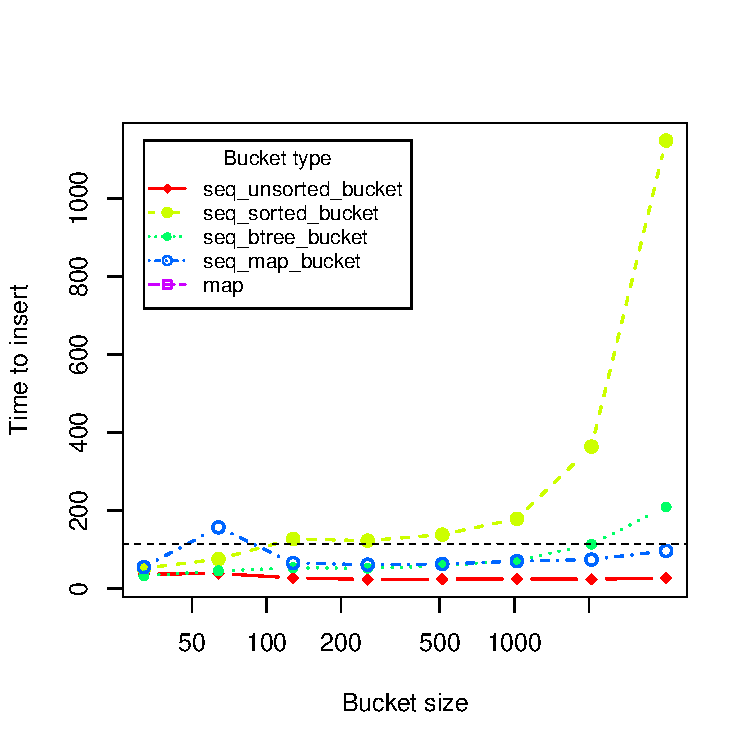
\includegraphics[width=1.0\textwidth]{plots/i7_30m_insert}
        }
        \subfloat[Search]{
            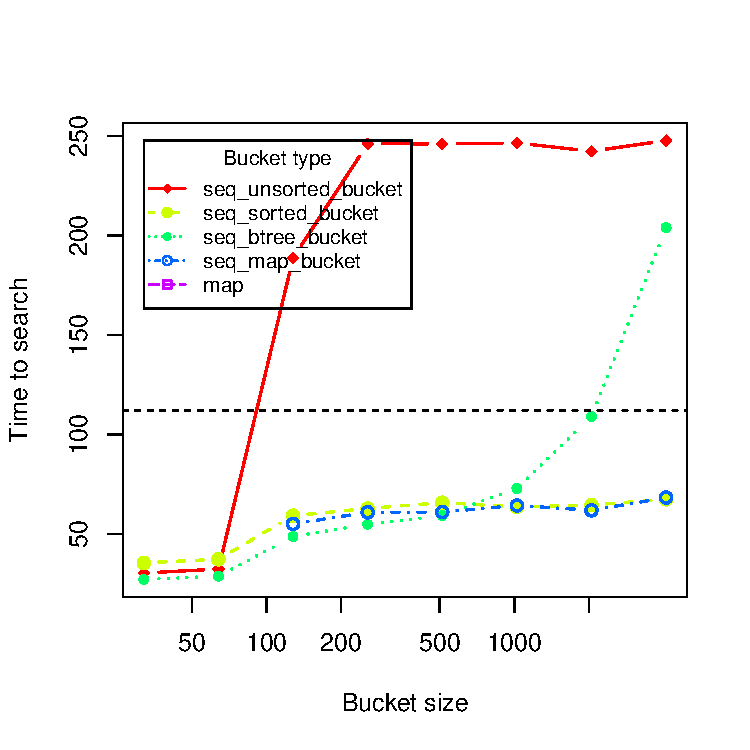
\includegraphics[width=1.0\textwidth]{plots/i7_30m_search}
        }
        \caption{Sequential test: Scaling of insertion and self-search times
        using the 30M Random dataset, with varying bucket sizes from 32 to
        4096. The {\keyword map} time is shown for reference as a dotted line.}
        \label{fig:seq_30m}
    \end{figure*}
\end{landscape}



\clearpage
\section{Parallel scaling}
In testing the parallel scaling of the different burst trie variants,
testing has been done on all three machines in order to evaluate scaling
to the number of CPUs.

The first improvement made was to the locking method of the nodes. Here in
Figure \ref{fig:globallock}, the difference is shown.
\begin{figure}[h!]
    \centering
    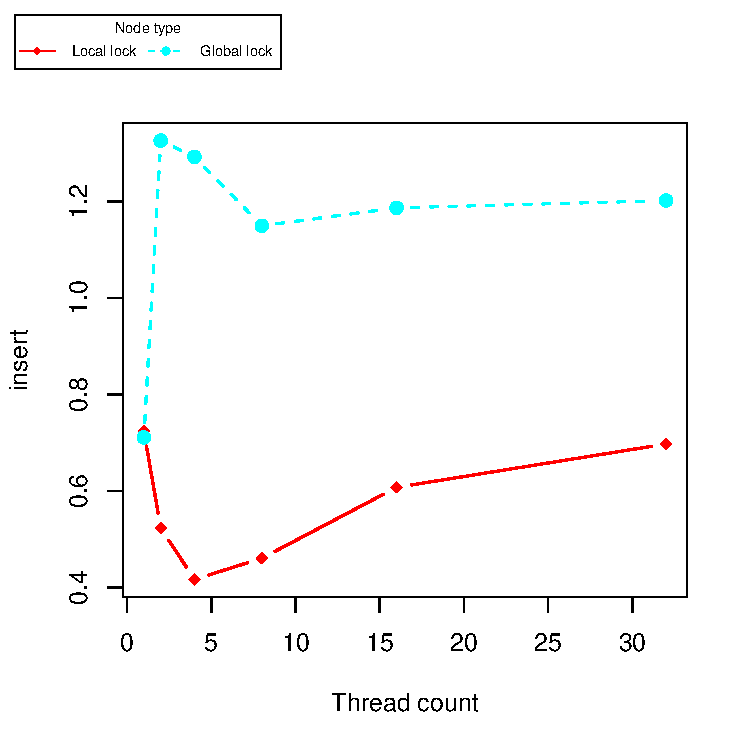
\includegraphics[width=0.5\textwidth]{plots/ts_locking}
    \fxwarning{Fix globallock plot}
    \caption{Thread scaling with global and local locking on the i7 machine (quad core),
    and the newsgroups dataset.}
    \label{fig:globallock}
\end{figure}
It is clear that the global lock is not a viable solution, these tests
show a clear bottleneck already beginning to show at 2 cores for insertions.
As such, insertions using more than a single thread are slower, since no
parallelism is gained, while synchronization of caches and locking is added.
The local locking on the other hand benefits from adding threads up to the
number of available CPUs.



While the sequential results show a clear tendency towards increased runtime
with larger containers, the sizes also influence the structure of the trie.
This means that different bucket sizes will scale differently.

\begin{table}[h]
    \centering
    \begin{tabular}[here]{ l l l l }
    \hline
        Bucket type            & Size & Insert & Search\\\hline
        %
        STL::Map               & 256  & 1.768  & 5.441\\
        Sorted dynamic array   & 256  & 3.301  & 5.261\\
        Unsorted dynamic array & 64   & 1.030  & 3.644\\
        Unsorted dynamic array & 128+ & ~0.600 & 6.108\\
        Binary tree            & 128  & 1.523  & 4.938\\
        Binary tree            & 32   & 0.979  & 5.680\\
    \hline
    \end{tabular}
    \caption{i7 30M: Best observed speedup factor for each bucket in the 30M
    dataset for up to 32 threads on the i7 quad-core machine (virtual
    octo-core). Results shown as best insertion time and best search time. The
    same size performed best on both if there is only one line.}
    \label{tab:speedups_30m_i7}
\end{table}
\begin{table}[h]
    \centering
    \begin{tabular}[here]{ l l l l }
    \hline
        Bucket type            & Size & Insert & Search\\\hline
        %
        STL::Map               & 128  & 1.054  & 2.120\\
        STL::Map               & 4096 & 0.702  & 2.564\\
        Sorted dynamic array   & 32   & 1.584  & 2.533\\
        Sorted dynamic array   & 4096 & 0.825  & 2.970\\
        Unsorted dynamic array & 64   & 1.065  & 2.177\\
        Unsorted dynamic array & 4096 & 0.603  & 3.941\\
        Binary tree            & 1024 & 1.714  & 2.218\\
        Binary tree            & 4096 & 1.293  & 2.530\\
    \hline
    \end{tabular}
    \caption{i7 Shakespeare: Best observed speedup factor for each bucket in
    the shakespeare dataset for up to 32 threads on the i7 quad-core machine
    (virtual octo-core). Results shown with best insertion time and best search
    time. The same size performed best on both if there is only one line.}
    \label{tab:speedups_shsp_i7}
\end{table}

The results from the 30M dataset (table \ref{tab:speedups_30m_i7} and page
\pageref{fig:ts_i7_30m}) show that it
is possible to obtain speedup factors of up to $6.1$ with a fully concurrent
locking mechanism on an octo-core system. With this as the reference, the gains of
a factor $3.3$ on insertions and a factor $5.2$ on searches for the sorted dynamic
arrays seem respectable. The sorted dynamic array with a size of 256 is the
only structure/size combination that scales well on both insertion and search. The
four virtual cores (Hyper-threading) have a greater impact on performance than
expected, with most tests scaling up to 8 threads. The scaling of the i7 is
high enough, that the results from the Xeon setup have been discarded due to
inconsistencies from uncontrolled load factors. The scaling of the two resp.
four cores can be seen in on page \pageref{fig:ts_shsp}.

The greatest gains appearing from unsorted array concurrency is evidence that
the locking favors heavy work in the leaves. This fits perfectly with the
expected node-level parallelism, which also explains why the greatest gains in
insertion is seen with sorted arrays, being the only bucket structure with
linear insertion times, and thereby up to $O(b^2)$ bursting times.

It is somewhat surprising that the searches take such a big hit from the
locking, seen in the larger unsorted array cases, and when comparing with
the shakespeare set (table \ref{tab:speedups_shsp_i7}). The shakespeare tests
result in a much smaller trie, and the continuous scaling of the trie (seen in
Table \ref{tab:bncount_shakespeare}) allows us to conclude that the overhead
from locks is dominant for smaller containers. This is seen by all containers
favoring larger buckets, meaning a shallower trie and less locks. The results
for the shakespeare and newsgroup sets show the same conclusion, the scaling
    can be seen on page \pageref{fig:ts_i7_nsgrp}.

The empirical concurrency of the read-locks is hereby reduced. The difference
is even greater on the Xeon machine, where the maximum speedup factor observed
for searching was $4.1$ for the 30M set. The Xeon results are very inconsistent
    due to shared resources with other students, and have been only used for
    reference.

\chapter{Conclusion}

% Parallelising the trie
Using a relatively simple locking mechanism, speedups of up to a factor $6$
were observed for searches and $3.5$ for insertions, when utilizing 8
processors. These were observed for two different bucket types, sorted
and unsorted arrays of size 256.

The best times are obtained with large unsorted arrays if the structure is
used in a search-intensive environment. If the operations are equally
distributed, the best results were obtained with binary tree buckets of size 32.
Here the structure is built in 18 seconds and searched in 10, using 4 threads,
compared to the best sequential times of 43 and 32 seconds for an unsorted
array bucket with a size of 32.


In theory the read-locks allow full concurrency, and as such linear scaling to the
processor count was expected. The results show that the one lock per node
approach is not a globally suited solution, since the scaling is very dependent
on the height of the trie. The searches favoring unsorted buckets is an indication
that the node-level parallelism is the bottleneck, allowing the biggest portion
of the work to be done in the leaves.

For insertions the exclusive locking comes at the cost of negative speedup for
over-saturated processors due to synchronization, and when combined with very
efficient bucket operations becomes the dominant factor for larger tries.

The waiting itself is the problem for smaller tries, since the locking is
incremental from the root down, creating what is essentially a sequential
locking queue at the root. In order to obtain increased parallelism smaller
bucket sizes are used to increase the size of the trie. At the same time,
searches scale the best with large containers, since the locking overhead
is minimized by spending more time in the buckets.
This leads to the conclusion that a lock-free implementation is the only
way to make the trie scale better on insertions, without compromising
the search efficiency.

The lock-free solution was attempted implemented, but without success.
Therefore, no empirical results are available for the lock-free solution.

\section{Future work}
Recommended smaller optimizations from the current implementation:
Avoiding the linear scan of the {\keyword max/min} index updates by using
bitvectors, and using constant-time burst insertions for sorted arrays.

A caveat of the chosen implementation is the lack of a reduction criteria
for removals beyond the naive. Such a criteria will be able to guarantee
that a reduction is only one level at a time. This is expected to  make
reasoning about a lock-free removal solution easier.

The implementation of a lock-free trie was unsuccessful, and remains a
theoretical possibility. The theoretical ground work has been laid for
implementing a wait-free trie, both with and without assisted bursting.
A successful implementation of this is a promising next step in the
parallelisation of the burst trie.

If such a structure is implemented, the perceived locking granularity of each
node will be increased by a factor of $\alpha$, as a result of backing-off on
concurrent changes of the same memory location. No locking actually occurs,
and the resulting structure can scale to any number of processors.
The proposed structure only covers the targetted operations of inserting
and searching. The added STL functionalities of iteration and removal
have not been covered in the proposed lock-free trie. This could be the
focus for future work on the lock-free trie.

%% Implementing the trie
%In extending the structure to support even simple removals, an extra counter
%was added to the nodes and the buckets. The implemented removal method
%is simplistic to avoid maintaining extra size counts. This has the drawback of
%allowing long chains of nodes to remain, when they could be reduced to a bucket.
%
%The operations required by an STL {\keyword (Multi-)map} have been implemented:
%
%For efficient iterators, the buckets are made into a linked list, adding two
%pointers per bucket. These are maintained in $O(h+\alpha)$ time in the chosen
%implementation.
%
%In order to minimize the linear scanning, {\keyword min} and {\keyword max}
%indices are added to the nodes. These are maintained in $O(\alpha)$, by
%scanning the children array. The more efficient solution of bitvectors has not
%been implemented, which would allow this to be reduced to constant work.
%
%The linked list of buckets is also used for finding the predecessor and
%successor to a given element, scanning the bucket. If no bucket is found
%linear scanning of the children array is performed, until one is found.
%As such these methods come for free when the iterators have been implemented.
%
%The differences between a set and a map is only one of inserting pointers together
%with the keys. As such no changes are required. The only difference between a
%map and a multi-map is made in the buckets. If a multi-map is desired, the
%buckets need to insert a new key regardless of preexisting keys. If a map/set is
%wanted, the buckets need to determine if the key already exists.
%The implemented structure does not include this check, and is therefore
%a multi-map.
%\\

\bibliographystyle{plain}
\bibliography{bibliography}
\chapter{Appendix}
\begin{landscape}
% i7 !!
\begin{figure}[H]
    \subfloat[Insertion time] {
        \includegraphics[width=1.0\textwidth]{plots/i7/plot_0_ts_sorted_bucketinsert}
    }
    \subfloat[Search] {
        \includegraphics[width=1.0\textwidth]{plots/i7/plot_0_ts_sorted_bucketsearch}
    }
    \label{fig:ts_i7_30m_sorted}
    \caption{Multithreaded scaling of the sorted dynamic array bucket with varying sizes on the
    i7 machine (4 cores). Testing done with the 30M dataset.}
\end{figure}
\begin{figure}[H]
    \subfloat[Insertion time] {
        \includegraphics[width=1.0\textwidth]{plots/i7/plot_0_ts_unsorted_bucketinsert}
    }
    \subfloat[Search] {
        \includegraphics[width=1.0\textwidth]{plots/i7/plot_0_ts_unsorted_bucketsearch}
    }
    \label{fig:ts_i7_30m_unsorted}
    \caption{Multithreaded scaling of the unsorted dynamic array bucket with varying sizes on the
    i7 machine (4 cores). Testing done with the 30M dataset. Note that the smaller bucket size tests did not complete. This is caused by lack of memory.}
\end{figure}
\begin{figure}[H]
    \subfloat[Insertion time] {
        \includegraphics[width=1.0\textwidth]{plots/i7/plot_0_ts_map_bucketinsert}
    }
    \subfloat[Search] {
        \includegraphics[width=1.0\textwidth]{plots/i7/plot_0_ts_map_bucketsearch}
    }
    \label{fig:ts_i7_30m_map}
    \caption{Multithreaded scaling of the STL::Map bucket with varying sizes on the
    i7 machine (4 cores). Testing done with the 30M dataset.}
\end{figure}
\begin{figure}[H]
    \subfloat[Insertion time] {
        \includegraphics[width=1.0\textwidth]{plots/i7/plot_0_ts_btree_bucketinsert}
    }
    \subfloat[Search] {
        \includegraphics[width=1.0\textwidth]{plots/i7/plot_0_ts_btree_bucketsearch}
    }
    \label{fig:ts_i7_30m_btree}
    \caption{Multithreaded scaling of the binary tree bucket with varying sizes on the
    i7 machine (4 cores). Testing done with the 30M dataset.}
\end{figure}
% ask !!
\begin{figure}[H]
    \subfloat[Insertion time] {
        \includegraphics[width=1.0\textwidth]{plots/ask/plot_0_ts_sorted_bucketinsert}
    }
    \subfloat[Search] {
        \includegraphics[width=1.0\textwidth]{plots/ask/plot_0_ts_sorted_bucketsearch}
    }
    \label{fig:ts_ask_30m_sorted}
    \caption{Multithreaded scaling of the sorted dynamic array bucket with varying sizes on the
    ask machine (8 cores). Testing done with the 30M dataset.}
\end{figure}
\begin{figure}[H]
    \subfloat[Insertion time] {
        \includegraphics[width=1.0\textwidth]{plots/ask/plot_0_ts_unsorted_bucketinsert}
    }
    \subfloat[Search] {
        \includegraphics[width=1.0\textwidth]{plots/ask/plot_0_ts_unsorted_bucketsearch}
    }
    \label{fig:ts_ask_30m_unsorted}
    \caption{Multithreaded scaling of the unsorted dynamic array bucket with varying sizes on the
    ask machine (8 cores). Testing done with the 30M dataset.}
\end{figure}
\begin{figure}[H]
    \subfloat[Insertion time] {
        \includegraphics[width=1.0\textwidth]{plots/ask/plot_0_ts_map_bucketinsert}
    }
    \subfloat[Search] {
        \includegraphics[width=1.0\textwidth]{plots/ask/plot_0_ts_map_bucketsearch}
    }
    \label{fig:ts_ask_30m_map}
    \caption{Multithreaded scaling of the STL::Map bucket with varying sizes on the
    ask machine (8 cores). Testing done with the 30M dataset.}
\end{figure}
\begin{figure}[H]
    \subfloat[Insertion time] {
        \includegraphics[width=1.0\textwidth]{plots/ask/plot_0_ts_btree_bucketinsert}
    }
    \subfloat[Search] {
        \includegraphics[width=1.0\textwidth]{plots/ask/plot_0_ts_btree_bucketsearch}
    }
    \label{fig:ts_ask_30m_btree}
    \caption{Multithreaded scaling of the binary tree bucket with varying sizes on the
    ask machine (8 cores). Testing done with the 30M dataset.}
\end{figure}
% c2d !!
\begin{figure}[H]
    \subfloat[Insertion time] {
        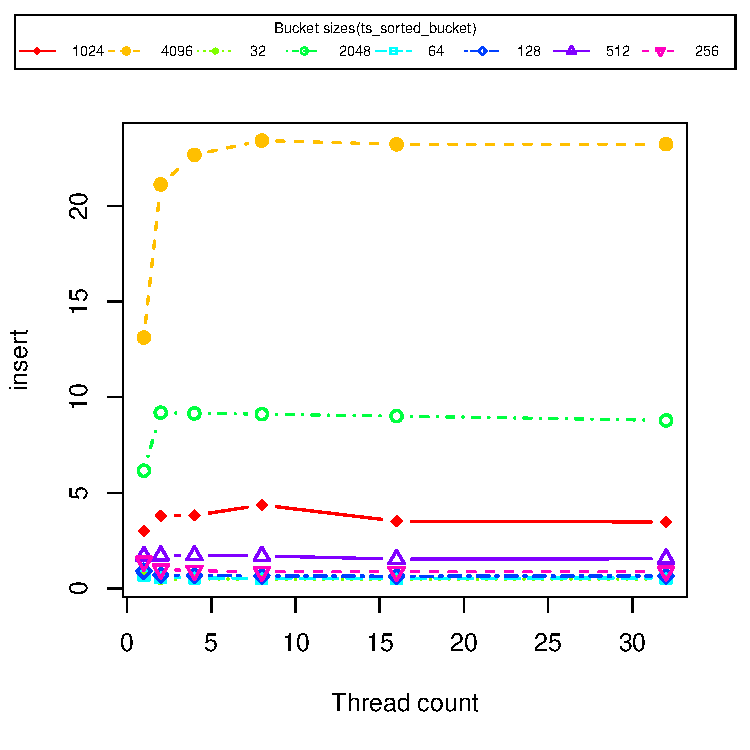
\includegraphics[width=1.0\textwidth]{plots/c2d/plot_1_ts_sorted_bucketinsert}
    }
    \subfloat[Search] {
        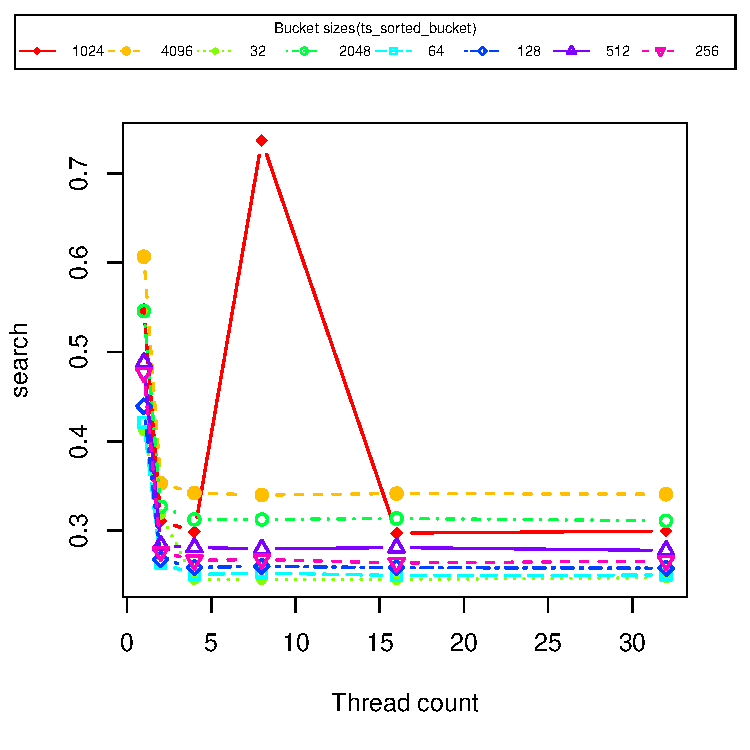
\includegraphics[width=1.0\textwidth]{plots/c2d/plot_1_ts_sorted_bucketsearch}
    }
    \label{fig:ts_c2d_shake_sorted}
    \caption{Multithreaded scaling of the sorted dynamic array bucket with varying sizes on the
    c2d machine (2 cores). Testing done with the shakespeare dataset.}
\end{figure}
\begin{figure}[H]
    \subfloat[Insertion time] {
        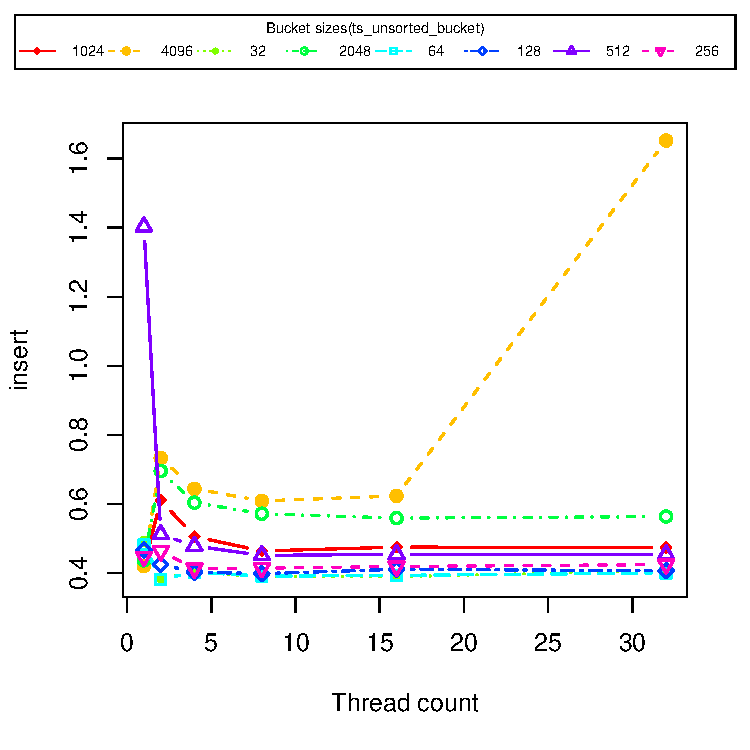
\includegraphics[width=1.0\textwidth]{plots/c2d/plot_1_ts_unsorted_bucketinsert}
    }
    \subfloat[Search] {
        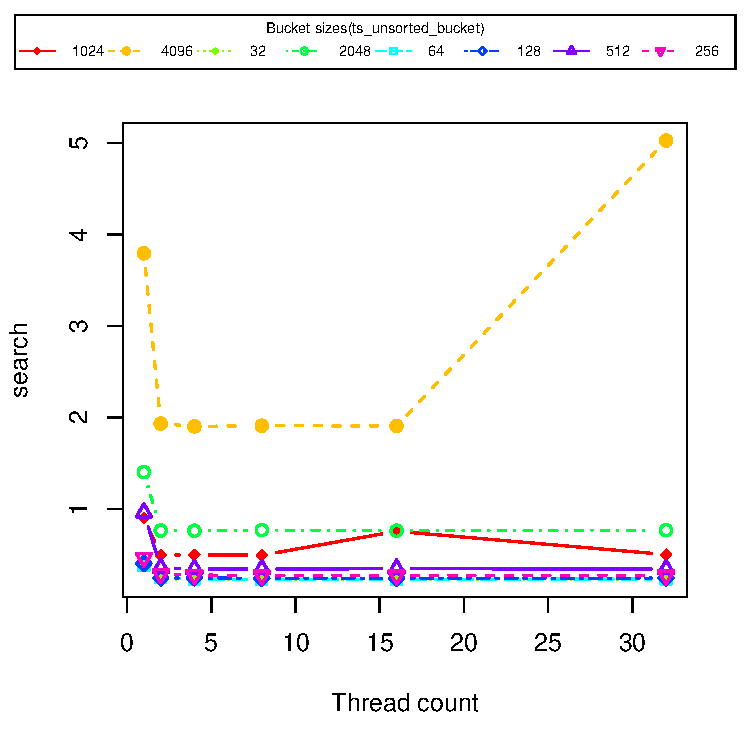
\includegraphics[width=1.0\textwidth]{plots/c2d/plot_1_ts_unsorted_bucketsearch}
    }
    \label{fig:ts_c2d_shake_unsorted}
    \caption{Multithreaded scaling of the unsorted dynamic array bucket with varying sizes on the
    c2d machine (2 cores). Testing done with the shakespeare dataset.}
\end{figure}
\begin{figure}[H]
    \subfloat[Insertion time] {
        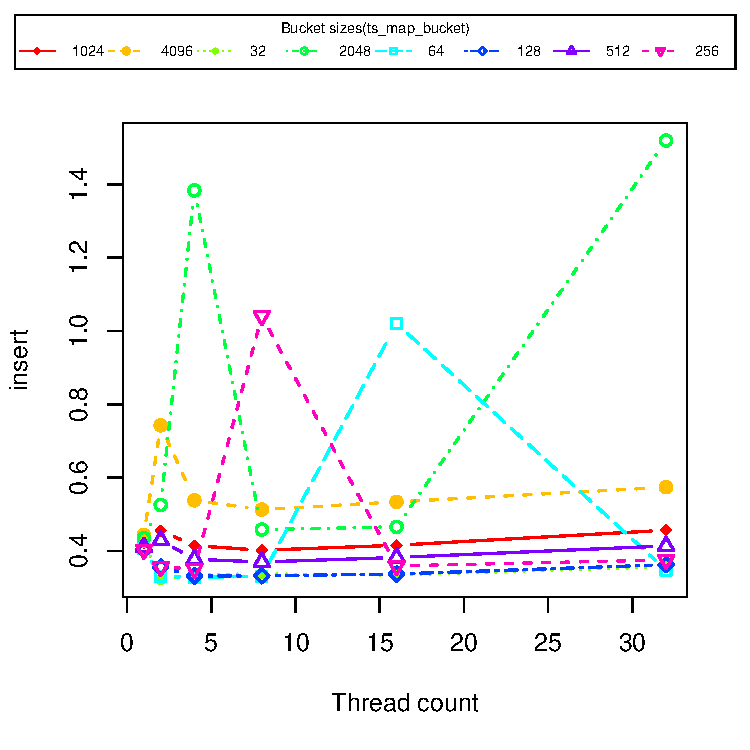
\includegraphics[width=1.0\textwidth]{plots/c2d/plot_1_ts_map_bucketinsert}
    }
    \subfloat[Search] {
        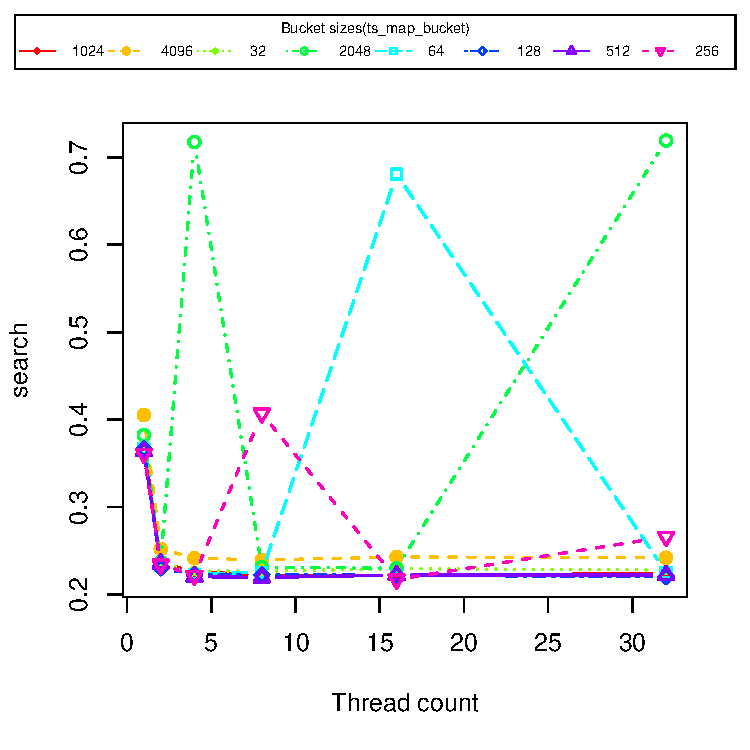
\includegraphics[width=1.0\textwidth]{plots/c2d/plot_1_ts_map_bucketsearch}
    }
    \label{fig:ts_c2d_shake_map}
    \caption{Multithreaded scaling of the STL::Map bucket with varying sizes on the
    c2d machine (2 cores). Testing done with the shakespeare dataset.}
\end{figure}
\begin{figure}[H]
    \subfloat[Insertion time] {
        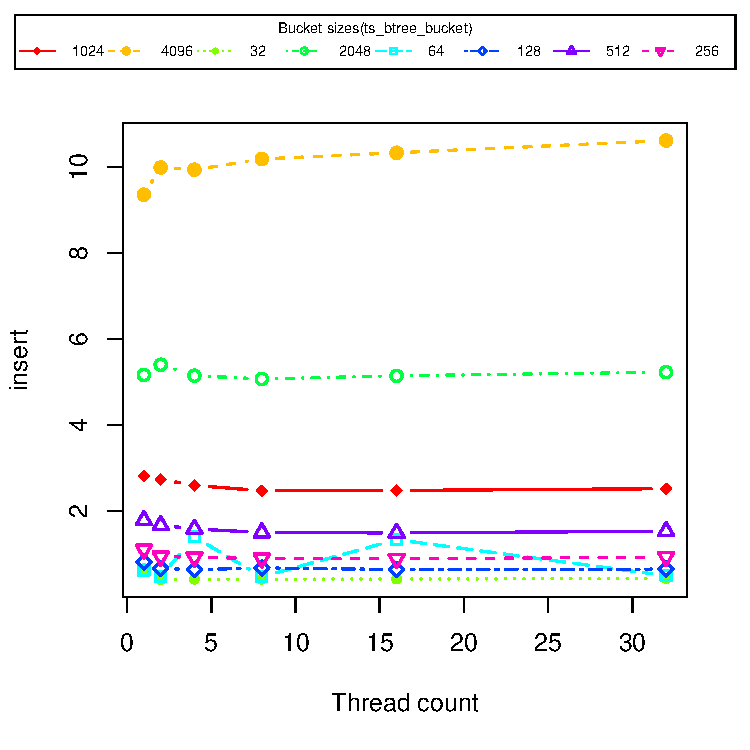
\includegraphics[width=1.0\textwidth]{plots/c2d/plot_1_ts_btree_bucketinsert}
    }
    \subfloat[Search] {
        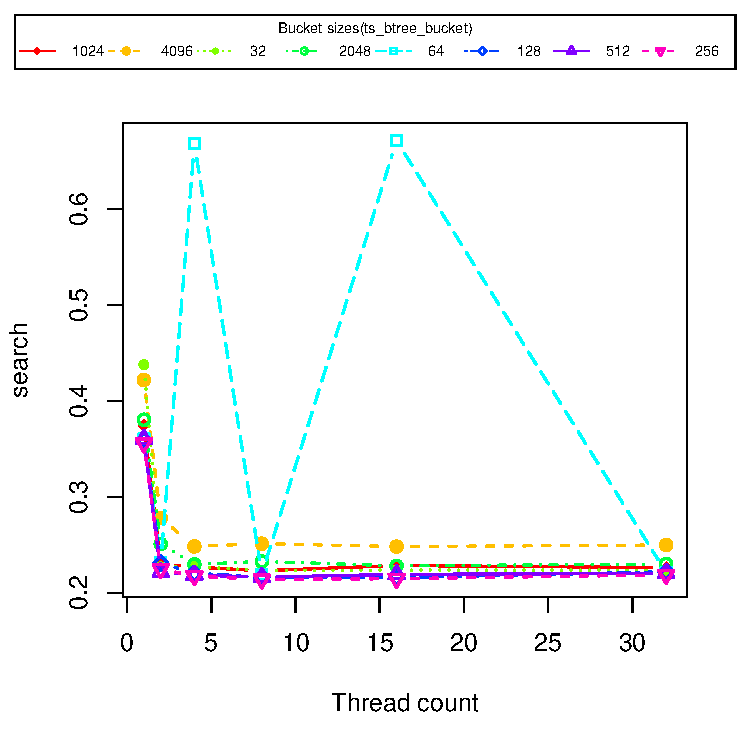
\includegraphics[width=1.0\textwidth]{plots/c2d/plot_1_ts_btree_bucketsearch}
    }
    \label{fig:ts_c2d_shake_btree}
    \caption{Multithreaded scaling of the binary tree bucket with varying sizes on the
    c2d machine (2 cores). Testing done with the shakespeare dataset.}
\end{figure}
% i7 !!
\begin{figure}[H]
    \subfloat[Insertion time] {
        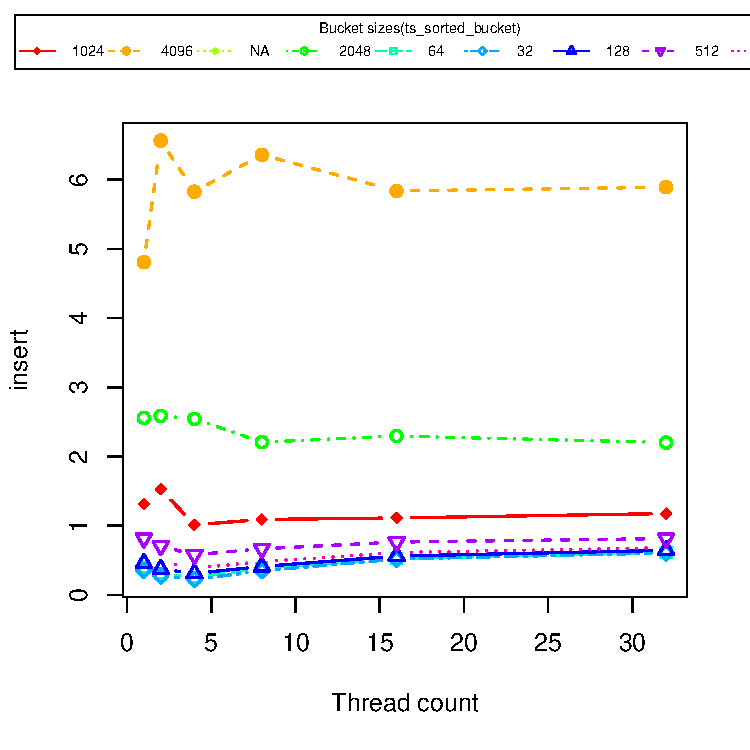
\includegraphics[width=1.0\textwidth]{plots/i7/plot_1_ts_sorted_bucketinsert}
    }
    \subfloat[Search] {
        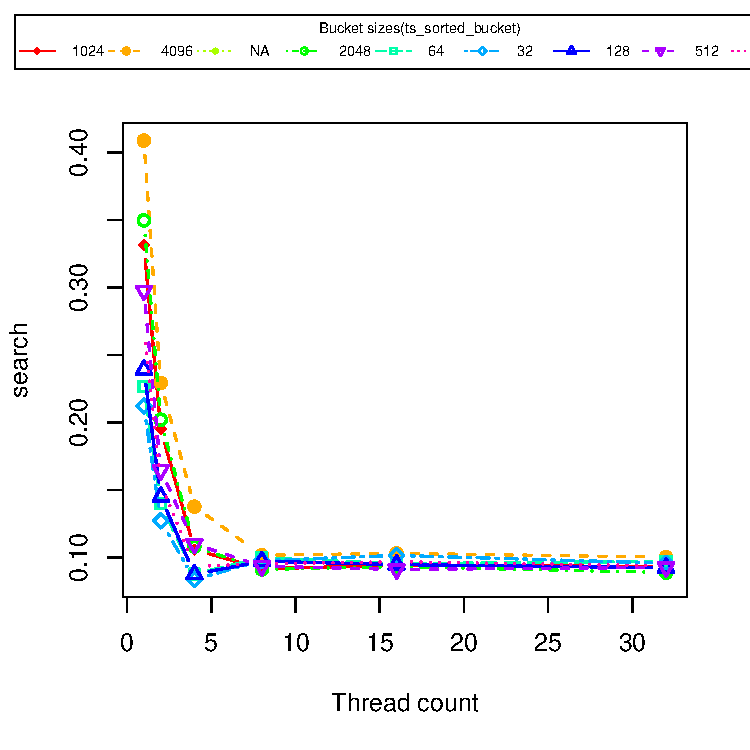
\includegraphics[width=1.0\textwidth]{plots/i7/plot_1_ts_sorted_bucketsearch}
    }
    \label{fig:ts_i7_shake_sorted}
    \caption{Multithreaded scaling of the sorted dynamic array bucket with varying sizes on the
    i7 machine (4 cores). Testing done with the shakespeare dataset.}
\end{figure}
\begin{figure}[H]
    \subfloat[Insertion time] {
        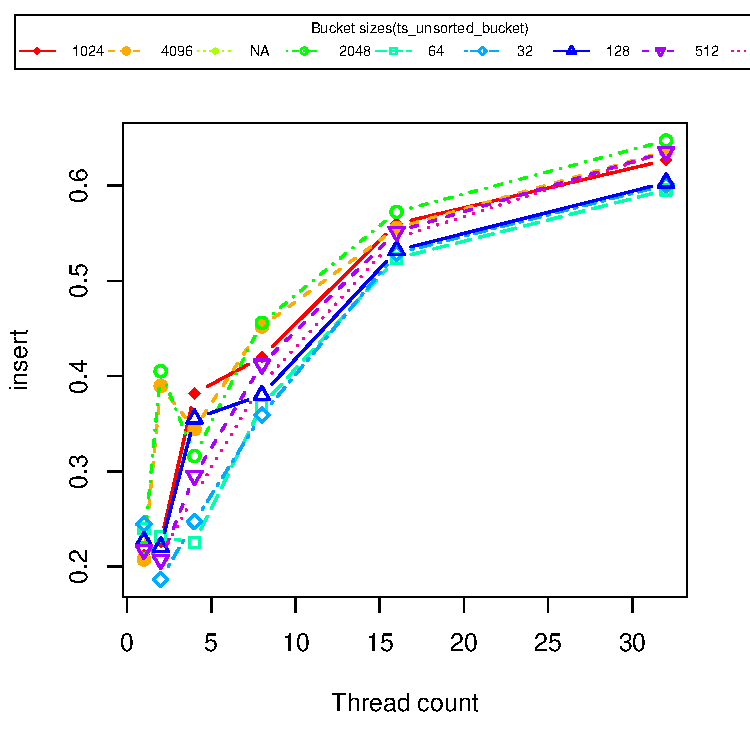
\includegraphics[width=1.0\textwidth]{plots/i7/plot_1_ts_unsorted_bucketinsert}
    }
    \subfloat[Search] {
        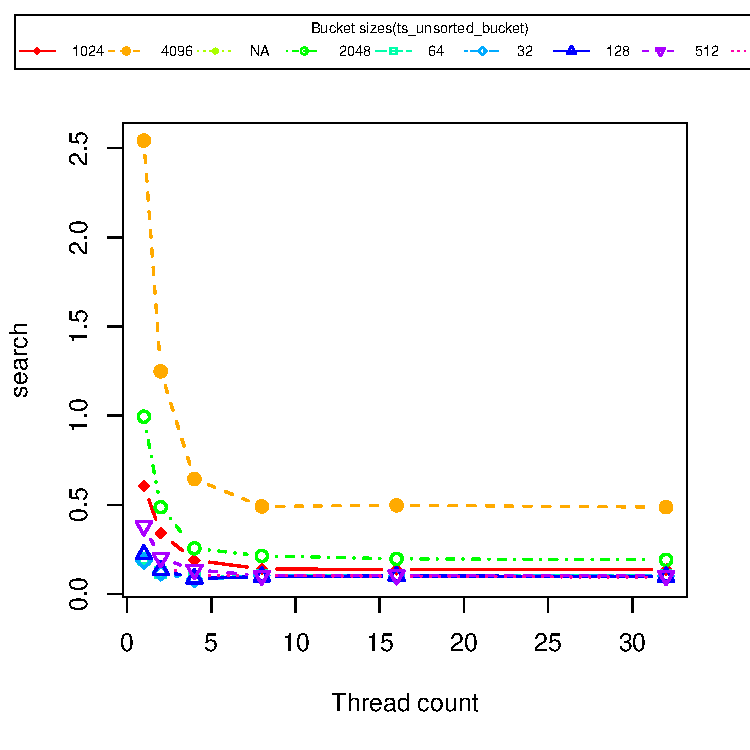
\includegraphics[width=1.0\textwidth]{plots/i7/plot_1_ts_unsorted_bucketsearch}
    }
    \label{fig:ts_i7_shake_unsorted}
    \caption{Multithreaded scaling of the unsorted dynamic array bucket with varying sizes on the
    i7 machine (4 cores). Testing done with the shakespeare dataset.}
\end{figure}
\begin{figure}[H]
    \subfloat[Insertion time] {
        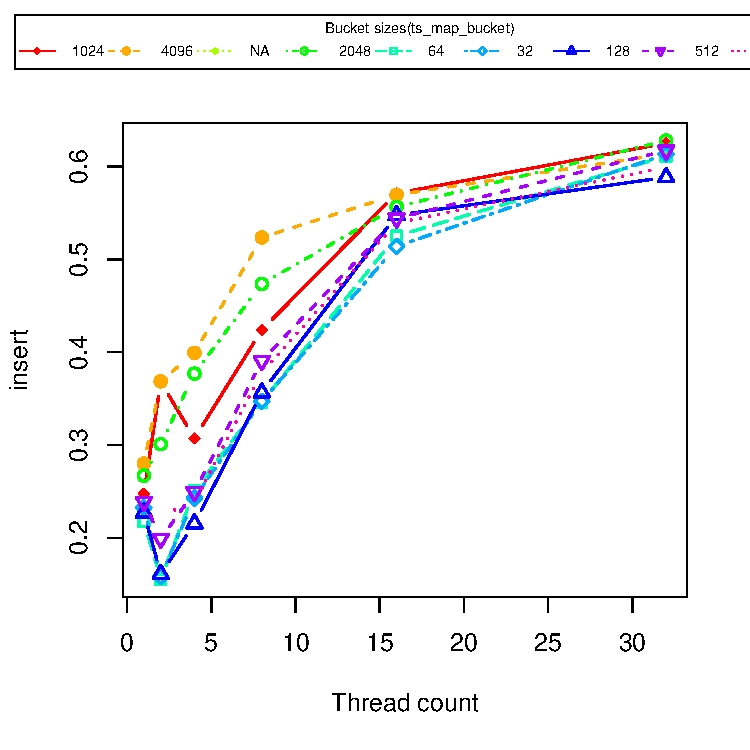
\includegraphics[width=1.0\textwidth]{plots/i7/plot_1_ts_map_bucketinsert}
    }
    \subfloat[Search] {
        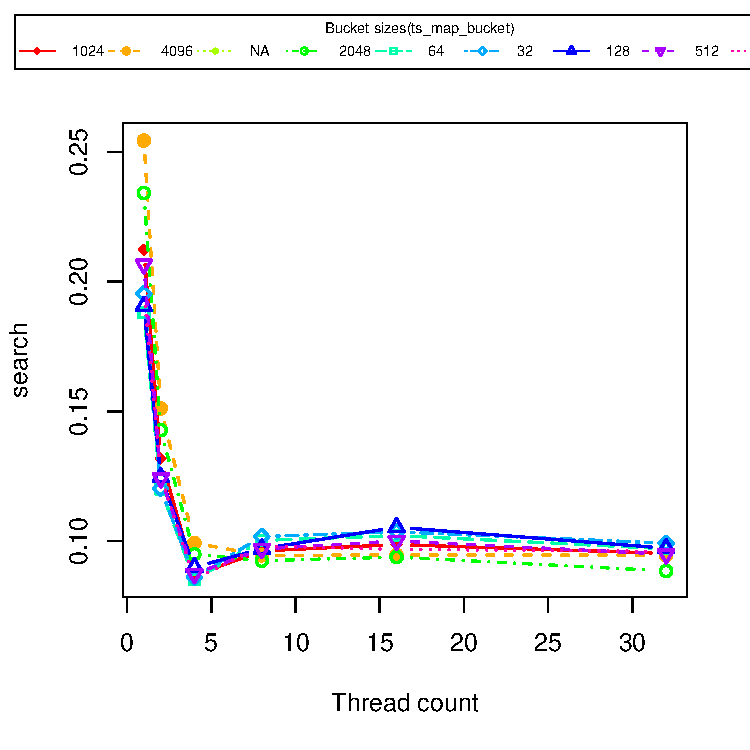
\includegraphics[width=1.0\textwidth]{plots/i7/plot_1_ts_map_bucketsearch}
    }
    \label{fig:ts_i7_shake_map}
    \caption{Multithreaded scaling of the STL::Map bucket with varying sizes on the
    i7 machine (4 cores). Testing done with the shakespeare dataset.}
\end{figure}
\begin{figure}[H]
    \subfloat[Insertion time] {
        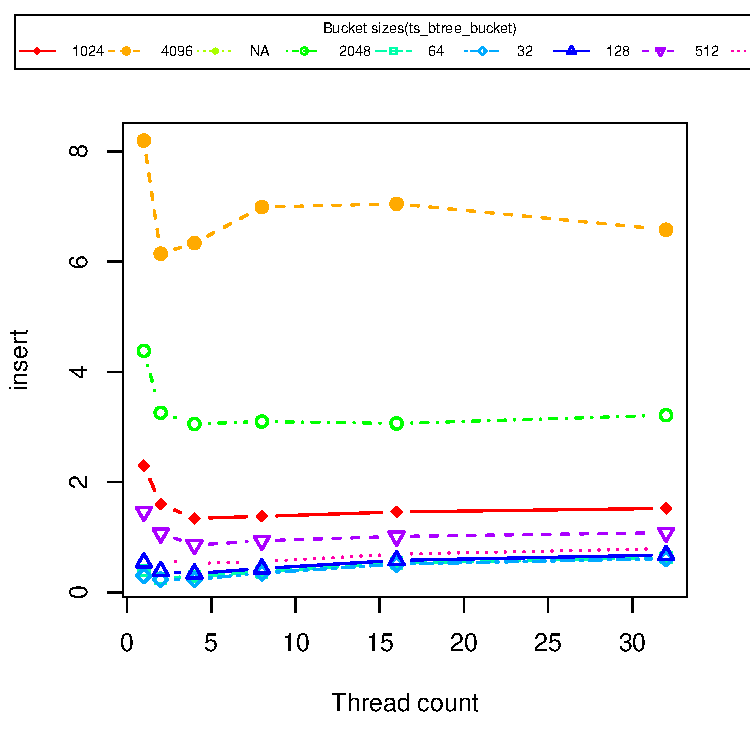
\includegraphics[width=1.0\textwidth]{plots/i7/plot_1_ts_btree_bucketinsert}
    }
    \subfloat[Search] {
        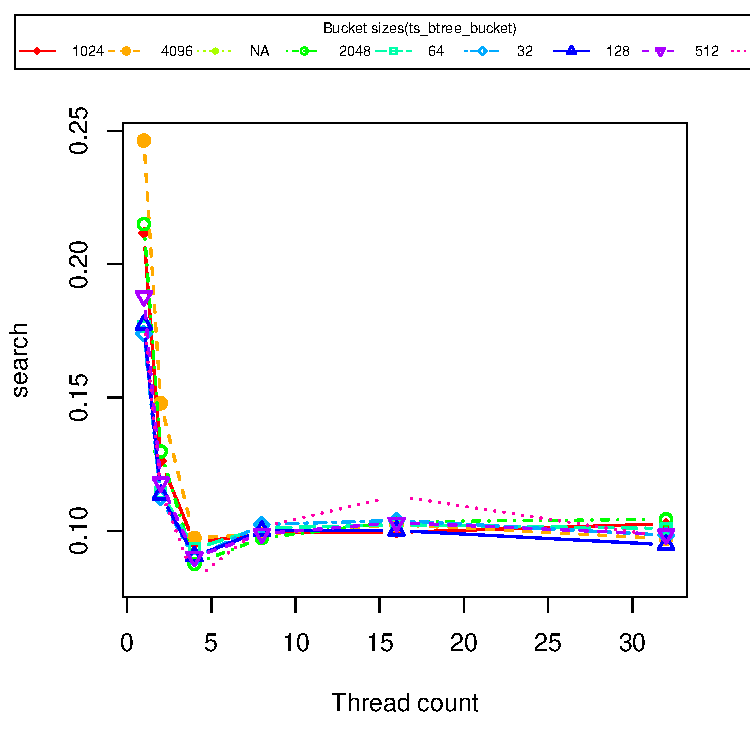
\includegraphics[width=1.0\textwidth]{plots/i7/plot_1_ts_btree_bucketsearch}
    }
    \label{fig:ts_i7_shake_btree}
    \caption{Multithreaded scaling of the binary tree bucket with varying sizes on the
    i7 machine (4 cores). Testing done with the shakespeare dataset.}
\end{figure}
\end{landscape}



\end{document}
